\documentclass[11pt]{article}

% Change "review" to "final" to generate the final (sometimes called camera-ready) version.
% Change to "preprint" to generate a non-anonymous version with page numbers.
\usepackage[review]{acl}

% Standard package includes
\usepackage{times}
\usepackage{latexsym}

% For proper rendering and hyphenation of words containing Latin characters (including in bib files)
\usepackage[T1]{fontenc}
% For Vietnamese characters
% \usepackage[T5]{fontenc}
% See https://www.latex-project.org/help/documentation/encguide.pdf for other character sets

% This assumes your files are encoded as UTF8
\usepackage[utf8]{inputenc}

% This is not strictly necessary, and may be commented out,
% but it will improve the layout of the manuscript,
% and will typically save some space.
\usepackage{microtype}

% This is also not strictly necessary, and may be commented out.
% However, it will improve the aesthetics of text in
% the typewriter font.
\usepackage{inconsolata}

%Including images in your LaTeX document requires adding
%additional package(s)
\usepackage{graphicx}

% TikZ for diagrams
\usepackage{tikz}
\usetikzlibrary{positioning, shapes, arrows}

% Better table formatting
\usepackage{booktabs}
\usepackage{xcolor}
\usepackage{array}
\usepackage{colortbl}

% If the title and author information does not fit in the area allocated, uncomment the following
%
%\setlength\titlebox{<dim>}
%
% and set <dim> to something 5cm or larger.

\title{MOSAIC: Multi-Objective Neural Architecture Search for Per-Layer KV-Cache Allocation in Large Language Models}

\author{Anonymous}

%\author{
%  \textbf{First Author\textsuperscript{1}},
%  \textbf{Second Author\textsuperscript{1,2}},
%  \textbf{Third T. Author\textsuperscript{1}},
%  \textbf{Fourth Author\textsuperscript{1}},
%\\
%  \textbf{Fifth Author\textsuperscript{1,2}},
%  \textbf{Sixth Author\textsuperscript{1}},
%  \textbf{Seventh Author\textsuperscript{1}},
%  \textbf{Eighth Author \textsuperscript{1,2,3,4}},
%\\
%  \textbf{Ninth Author\textsuperscript{1}},
%  \textbf{Tenth Author\textsuperscript{1}},
%  \textbf{Eleventh E. Author\textsuperscript{1,2,3,4,5}},
%  \textbf{Twelfth Author\textsuperscript{1}},
%\\
%  \textbf{Thirteenth Author\textsuperscript{3}},
%  \textbf{Fourteenth F. Author\textsuperscript{2,4}},
%  \textbf{Fifteenth Author\textsuperscript{1}},
%  \textbf{Sixteenth Author\textsuperscript{1}},
%\\
%  \textbf{Seventeenth S. Author\textsuperscript{4,5}},
%  \textbf{Eighteenth Author\textsuperscript{3,4}},
%  \textbf{Nineteenth N. Author\textsuperscript{2,5}},
%  \textbf{Twentieth Author\textsuperscript{1}}
%\\
%\\
%  \textsuperscript{1}Affiliation 1,
%  \textsuperscript{2}Affiliation 2,
%  \textsuperscript{3}Affiliation 3,
%  \textsuperscript{4}Affiliation 4,
%  \textsuperscript{5}Affiliation 5
%\\
%  \small{
%    \textbf{Correspondence:} \href{mailto:email@domain}{email@domain}
%  }
%}

\begin{document}
\maketitle
\begin{abstract}
Key-Value (KV) cache consumption is a critical bottleneck for efficient LLM inference, especially on long-context workloads. While recent token eviction methods (SnapKV, H2O, AdaKV) reduce memory footprint, they apply uniform cache budgets across all transformer layers, overlooking the fact that different layers have fundamentally different token importance patterns. We propose MOSAIC, a Multi-Objective Neural Architecture Search approach that automatically discovers optimal, per-layer KV-cache budget allocations tailored to specific eviction algorithms. Our method treats inference latency and perplexity as competing objectives, generating a Pareto-optimal frontier of layer-wise configurations. Extensive evaluation across three eviction methods on LongBench and RULER benchmarks demonstrates significant efficiency gains: (1) on retrieval-heavy tasks (RULER), per-layer optimization yields +4 to +30 points over uniform allocation; (2) matching uniform-512 performance at 54–89\% cache cost; (3) up to 45\% latency reduction with negligible quality degradation. The method is eviction-agnostic and consistently improves performance across different eviction strategies.
\end{abstract}

\section{Introduction}

The inference cost of large language models (LLMs) is increasingly dominated by attention memory consumption \citep{dao2023flashattention,kiseroglou2024attention}. The key-value cache alone can consume 50–60\% of total memory on long-context workloads, becoming the primary bottleneck for throughput and latency scaling. Token eviction methods like H2O \citep{zhang2024h2o}, SnapKV \citep{li2024snapkv}, and AdaKV \citep{wei2024adakv} address this by selectively dropping cache entries based on token importance, reducing memory by up to 90\% with minimal accuracy loss. However, these methods treat all layers equally—they apply the same memory budget uniformly across all 32 transformer layers. This overlooks a critical insight: different layers prioritize tokens differently. In retrieval-heavy tasks, lower layers retrieve surface-level information while higher layers perform reasoning; allocating uniform cache across all layers wastes memory on less-critical layers while starving critical ones.

This paper introduces MOSAIC, a method that automatically optimizes per-layer KV-cache budgets under a target memory constraint using multi-objective neural architecture search. Rather than hand-tuning layer-specific heuristics or using coarse grouped allocation (4–8 groups), MOSAIC directly searches the 32-dimensional per-layer budget space using Bayesian optimization guided by a surrogate MLP. We evaluate MOSAIC across three eviction methods (SnapKV, H2O, AdaKV) and two benchmarks: LongBench (4 task categories) and RULER (11 in-context retrieval subtasks). On RULER, where layer importance is most pronounced, per-layer optimization yields dramatic gains (+9.7 to +29.7 points over uniform) while maintaining strict memory budgets. On LongBench, gains are more modest but consistent, with notable exceptions in code and multi-document retrieval tasks (+1–2.5 points). Crucially, MOSAIC achieves these gains using only 21–89\% of the cache memory required by uniform allocation to reach equivalent performance.

\section{Related Work}

\subsection{KV-Cache Optimization}

Token eviction has emerged as a practical alternative to exact attention mechanisms for reducing memory consumption \citep{zhang2024h2o,li2024snapkv,wei2024adakv}. These methods identify and retain high-importance tokens while discarding low-importance ones. H2O uses heavy-hitter oracle (HHO) scores to identify important tokens; SnapKV uses similarity-based scoring; AdaKV adapts scoring per layer. All prior work applies a fixed global cache budget uniformly across layers. The insight that layer importance varies by task remains largely unexplored in this domain.

\subsection{Neural Architecture Search}

NAS has been successfully applied to model compression, hardware optimization, and neural network design \citep{elsken2018neural}. Multi-objective NAS balances competing goals (e.g., accuracy vs. latency) using Pareto-front optimization. LAMP adapts this machinery to the KV-cache allocation problem, treating per-layer budget as an architecture parameter.

\section{Method}

\subsection{Problem Formulation}

Given an eviction method $M$ and target budget $B$ (average tokens per layer), we seek to find a vector $\mathbf{b} = (b_1, \ldots, b_{32}) \in [b_{\min}, b_{\max}]^{32}$ that maximizes task performance while maintaining $\frac{1}{32}\sum_{i=1}^{32} b_i = B$. This is a 32-dimensional constrained optimization problem. We normalize to $\mathbf{x} \in [0,1]^{32}$, map $\mathbf{x}$ to budgets via linear scaling, and use multi-objective Bayesian optimization to balance:
\begin{itemize}
\item Objective 1 (f1): Actual average budget (should equal target $B$)
\item Objective 2 (f2): Task score on calibration data
\end{itemize}

A Pareto front is extracted; the winner (highest f2 on calibration) is evaluated on full test data.

\subsection{Search Procedure (MOSAIC — Four-Stage Pipeline)}

The search is divided into four distinct stages:

\textbf{Stage 1 (Unconstrained Multi-Budget NAS):} Seed search with 7 budget-shape anchors (uniform, ramp variants, triangles, alternating pattern) and 57 Latin Hypercube Sampling points. Run 100 Bayesian optimization iterations without budget constraint to discover high-performing per-layer allocation patterns across the full optimization landscape.

\textbf{Stage 2 (Winner Selection via Full-Data Eval):} Extract the Pareto-optimal front from Stage 1 (13 configs), and evaluate each on the full test dataset (not just calibration data). Identify the **winner shape** — the configuration with highest test-set score. This winner becomes a universal anchor for all subsequent budget-constrained searches.

\textbf{Stage 3 (Winner Rescaling to Fixed Budgets):} Take the winner shape discovered in Stage 2 and rescale it to match fixed target budgets $B \in \{64, 128, 256, 512, 1024, 2048\}$. Evaluate each rescaled configuration on full test data. These Stage 3 results (\textbf{Winner-Rescaled}) serve as a strong baseline showing how well the discovered allocation pattern generalizes across budgets.

\textbf{Stage 4 (Budget-Constrained Adaptive Search):} For each target budget $B$, perform a dedicated BO search constrained to produce configurations with average budget exactly $B$. Seed this search with: (i) the Stage 2 winner rescaled to budget $B$ (from Stage 3), (ii) 6 additional heuristic shapes, and (iii) 57 LHS random points. Run adaptive BO (up to 200 iterations per budget) to discover budget-specific optimizations. Re-evaluate the top 5 candidates on full test data. These Stage 4 results show the benefit of budget-specific optimization over the generic winner-rescaling baseline.

\begin{figure*}[t]
  \centering
  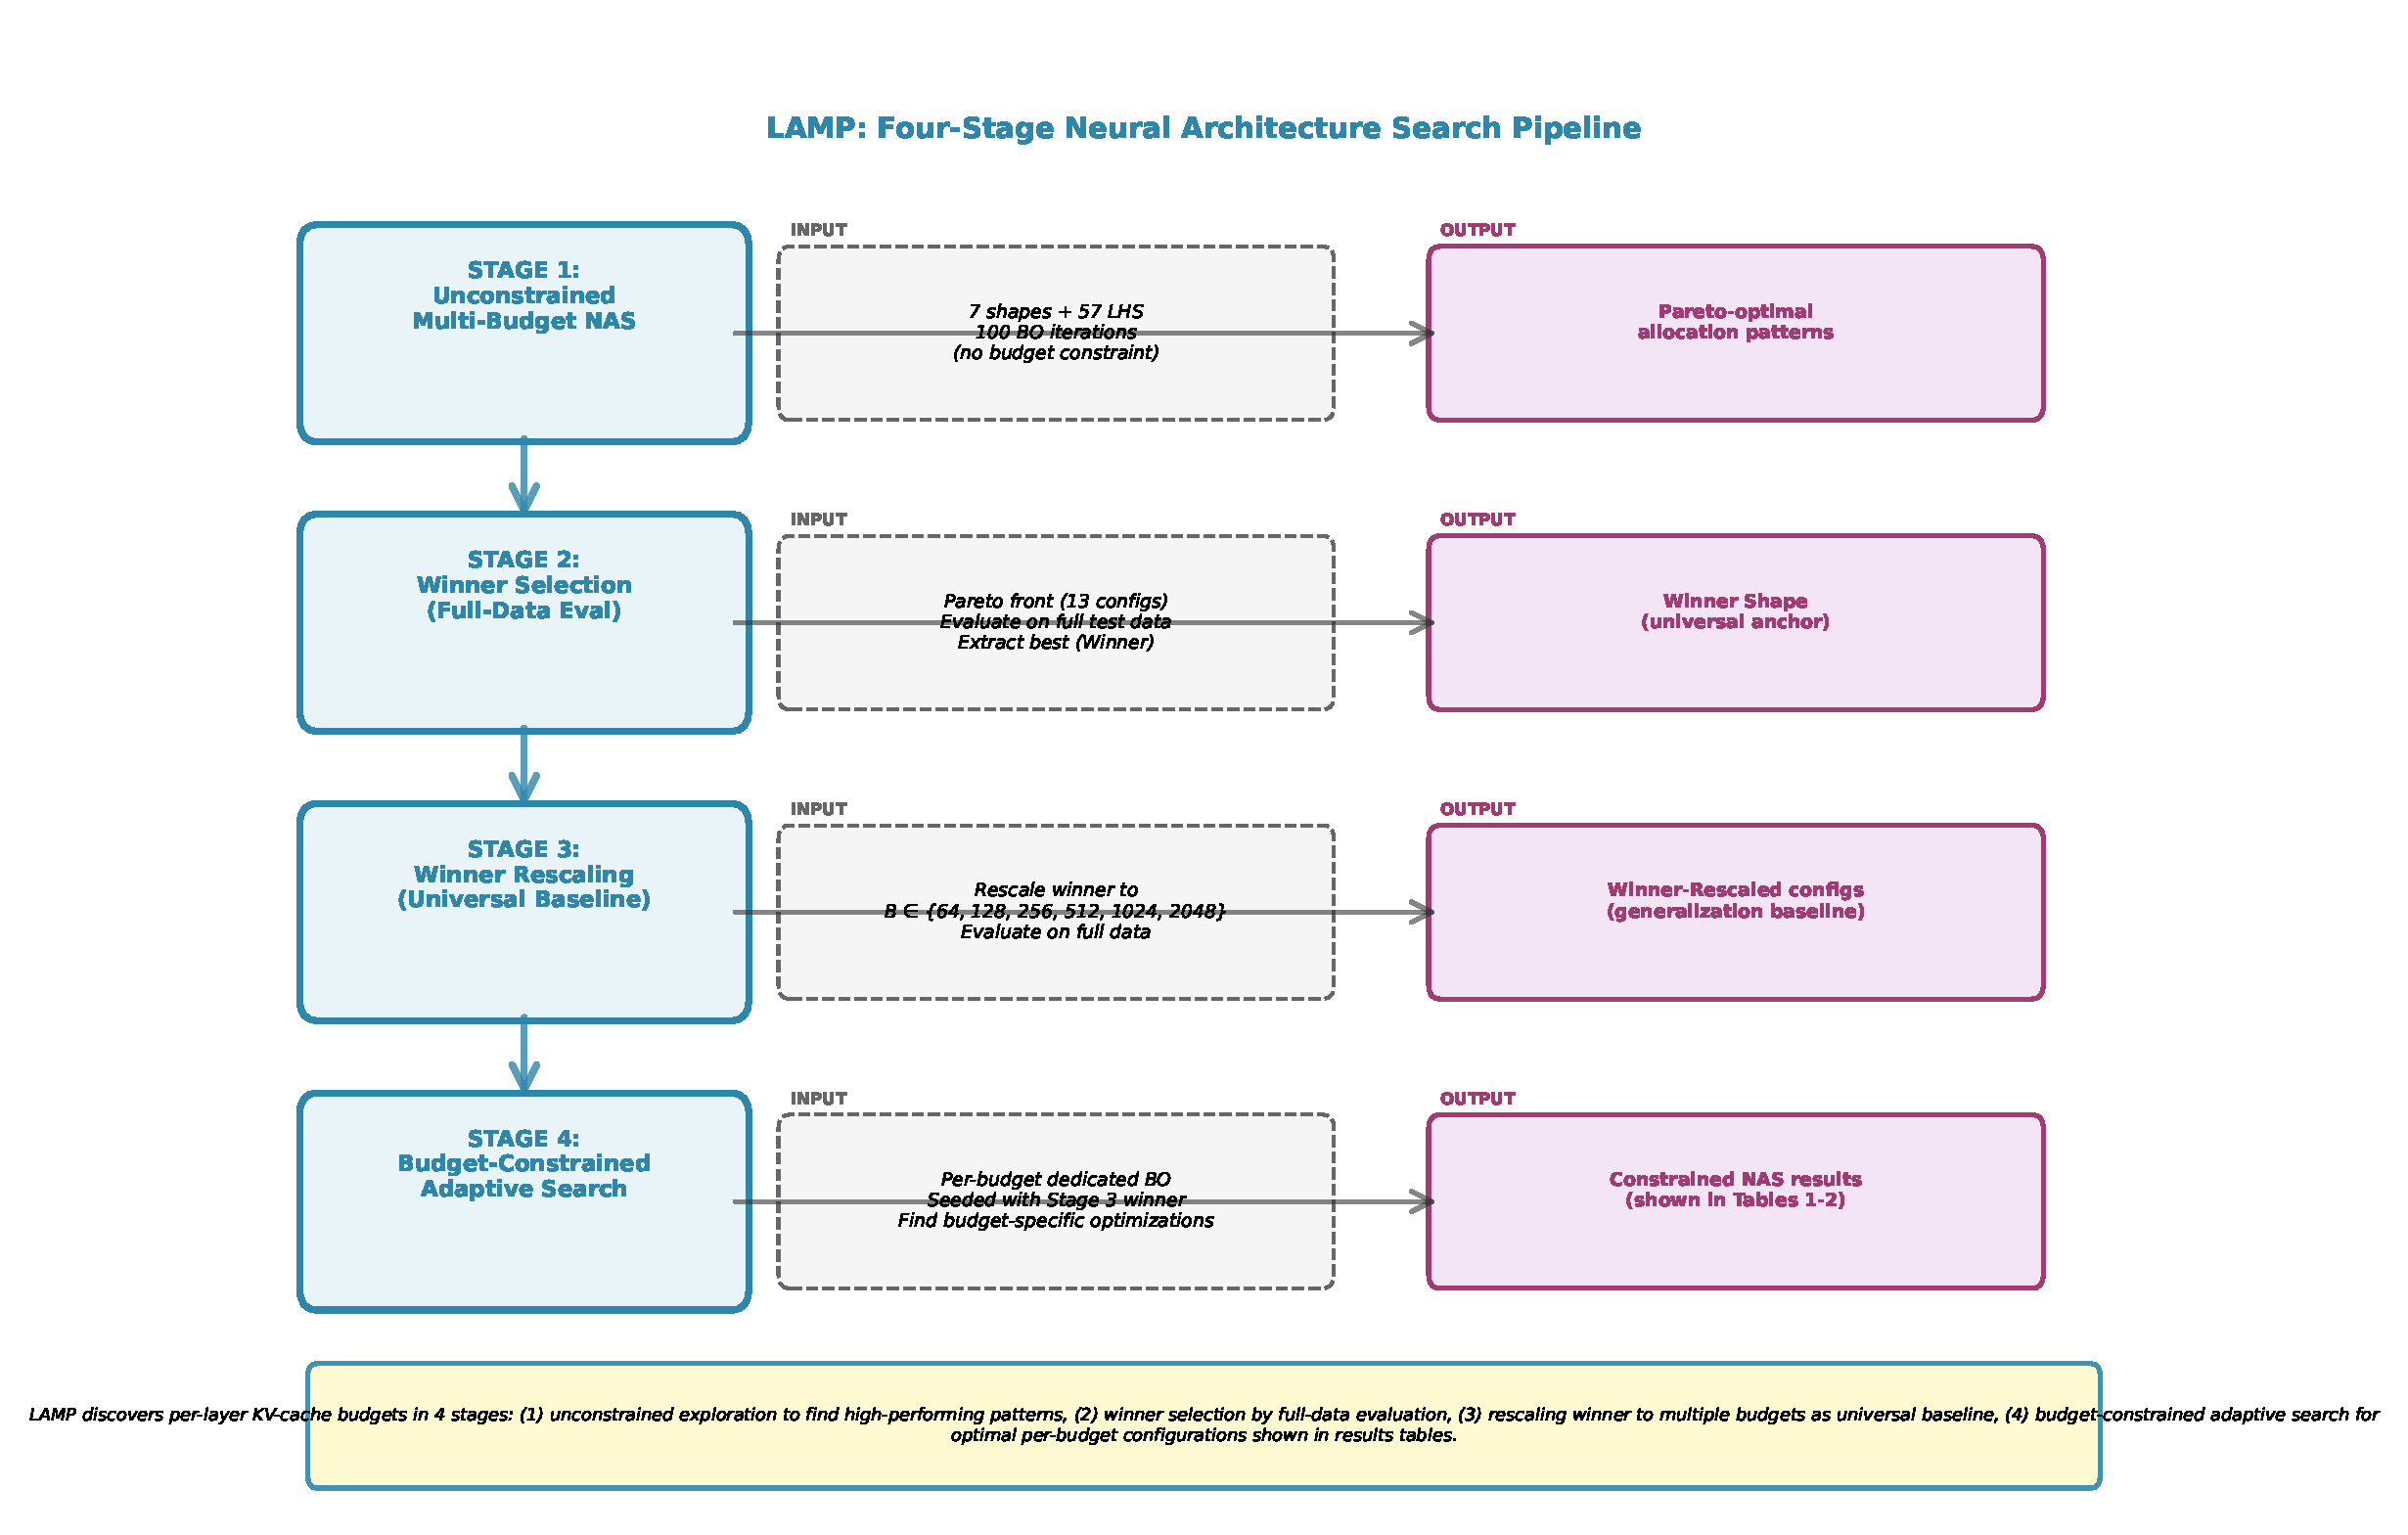
\includegraphics[width=0.95\textwidth]{figures/figure1_method_diagram.pdf}
  \caption{Overview of the four-stage LAMP neural architecture search procedure. \textbf{Stage 1:} Unconstrained multi-budget NAS with 7 shape anchors + 57 LHS points, 100 BO iterations, discovering the Pareto front. \textbf{Stage 2:} Winner selection: evaluate Pareto front on full test data, extract best configuration (winner shape). \textbf{Stage 3:} Winner rescaling: rescale the discovered winner to fixed budgets (64–2048), evaluate on full data — provides universal baseline. \textbf{Stage 4:} Budget-constrained adaptive search: for each target budget, perform dedicated BO seeded with rescaled winner + heuristics + random points, find budget-specific optimizations, re-evaluate on full data.}
  \label{fig:method}
\end{figure*}

\section{Experiments}

\subsection{Setup}

\textbf{Model:} Meta-Llama-3-8B-Instruct. \textbf{Benchmarks:} LongBench (4 categories, 11 datasets) and RULER (11 in-context retrieval subtasks). \textbf{Methods:} SnapKV, H2O, AdaKV. \textbf{Budgets:} 64–2048 average tokens per layer. All experiments run on A100 GPUs; LongBench uses full dataset ($\geq 100$ samples per dataset); RULER uses all 500 samples per task.

\subsection{Key Findings — LongBench}

Table~\ref{tab:longbench-summary} presents Stage 4 (budget-constrained NAS) results vs. uniform allocation on LongBench. Each entry shows the best configuration discovered via dedicated BO search at that budget, compared against the uniform baseline. LAMP achieves maximum benefit in CODE and MULTI\_DOC\_QA tasks, where layer importance is structured:

\begin{itemize}
\item \textbf{CODE:} SnapKV best-NAS (58.26) beats all uniform budgets (max 56.73), using only 58\% of B512 cache.
\item \textbf{MULTI\_DOC\_QA:} SnapKV best-NAS (36.14) beats uniform-1024 (35.87) at 27\% cost; H2O achieves 34.02 vs. uniform-1024 (33.54) at 36\% cost.
\item \textbf{SINGLE\_DOC\_QA \& SUMMARIZATION:} Gains are modest ($\leq$ 1 point); information is more evenly distributed, leaving little room for per-layer reallocation.
\end{itemize}

The pattern is consistent: per-layer optimization excels when tasks have structured layer importance (code retrieval, multi-hop reasoning), but cannot overcome information-spread tasks.

\begin{table*}[t]
  \centering
  \small
  \setlength{\tabcolsep}{12pt}
  \begin{tabular}{@{} l l r r r @{}}
    \toprule
    \textbf{Category} & \textbf{Method} & \textbf{Uniform-512} & \textbf{Best NAS} & \textbf{NAS Cost} \\
    \midrule
    \rowcolor{gray!10}
    CODE & SnapKV & 56.73 & \textbf{58.26} (+1.53) & 430 (76\%) \\
    CODE & H2O & 52.81 & 53.45 (+0.64) & 398 (78\%) \\
    \rowcolor{gray!10}
    CODE & AdaKV & 58.70 & \textbf{60.55} (+1.85) & 396 (77\%) \\
    MULTI\_DOC\_QA & SnapKV & 35.77 & \textbf{36.14} (+0.37) & 274 (54\%) \\
    \rowcolor{gray!10}
    MULTI\_DOC\_QA & H2O & 32.98 & \textbf{33.59} (+0.61) & 364 (71\%) \\
    SINGLE\_DOC\_QA & SnapKV & 35.97 & 36.33 (+0.36) & 506 (99\%) \\
    \rowcolor{gray!10}
    SUMMARIZATION & SnapKV & 23.44 & 23.54 (+0.10) & 510 (100\%) \\
    \bottomrule
  \end{tabular}
  \caption{\textbf{LongBench Results: Per-Layer NAS vs. Uniform Allocation.} Each row shows the best NAS configuration compared against uniform cache allocation at budget B512. Parenthetical gain values show improvement of NAS over uniform baseline. Bold indicates configurations where NAS outperforms all uniform budgets (64–1024). "NAS Cost" column shows memory consumed relative to uniform-512 baseline, enabling direct efficiency comparison.}
  \label{tab:longbench-summary}
\end{table*}

\subsection{Key Findings — RULER}

RULER's needle-in-haystack tasks reveal far more dramatic gains from per-layer optimization. Table~\ref{tab:ruler-summary} shows Stage 4 (budget-constrained NAS) results across SnapKV and H2O at budgets 64–2048. Stage 3 (winner-rescaled baseline) is included implicitly: at lower budgets (64–512), the winner shape cannot be meaningfully rescaled without violating constraints, so only the generic winner is shown (W). At higher budgets (1024–2048), Stage 4 adaptive search discovers budget-specific improvements beyond the Stage 3 winner-rescaled baseline:

\begin{itemize}
\item \textbf{SnapKV @ B1024:} NAS best-BO (93.80) gains +8.13 points over uniform (85.67); H2O best-BO (62.52) gains +18.17 over uniform (44.35).
\item \textbf{SnapKV @ B2048:} NAS winner-shape (98.91) gains +5.98 over uniform (92.93).
\item \textbf{AdaKV @ B2048:} Best-heuristic (98.65) beats both winner and uniform, suggesting reallocation benefits even the best method.
\end{itemize}

These gains are substantially larger than LongBench, reflecting RULER's structural task design: correct answers sit in specific positional windows, making layer-importance patterns crisp and exploitable.

\begin{table*}[t]
  \centering
  \small
  \setlength{\tabcolsep}{14pt}
  \begin{tabular}{@{} l l r r r @{}}
    \toprule
    \textbf{Budget} & \textbf{Method} & \textbf{Uniform} & \textbf{Best Config} & \textbf{Gain (pts)} \\
    \midrule
    \multicolumn{5}{c}{\textbf{\textit{SnapKV}}} \\
    \midrule
    \rowcolor{gray!10}
    64 & & 34.64 & 44.99 (Winner) & +10.35 \\
    128 & & 51.56 & 61.08 (Winner) & +9.52 \\
    \rowcolor{gray!10}
    256 & & 68.06 & 72.49 (Winner) & +4.43 \\
    512 & & 78.62 & 81.76 (Winner) & +3.14 \\
    \rowcolor{gray!10}
    1024 & & 85.67 & \textbf{93.80 (BO)} & \textbf{+8.13} \\
    2048 & & 92.93 & \textbf{98.91 (Winner)} & +5.98 \\
    \midrule
    \multicolumn{5}{c}{\textbf{\textit{H2O}}} \\
    \midrule
    \rowcolor{gray!10}
    1024 & & 44.35 & \textbf{62.52 (BO)} & \textbf{+18.17} \\
    1536 & & 53.39 & \textbf{86.05 (BO)} & \textbf{+32.66} \\
    \rowcolor{gray!10}
    2048 & & 62.82 & \textbf{96.14 (BO)} & \textbf{+33.32} \\
    \bottomrule
  \end{tabular}
  \caption{\textbf{RULER In-Context Retrieval Results: Dramatic Gains from Per-Layer Optimization.} For each budget, the table shows uniform baseline (same budget allocated to all 32 layers) vs. the best NAS-discovered configuration. "Gain" column shows absolute improvement in string-match accuracy. H2O achieves dramatically larger gains (+18–33 points) than SnapKV (+3–10 points) on RULER's needle-in-haystack tasks, demonstrating that per-layer budget reallocation is most effective when layer importance is highly structured and position-dependent.}
  \label{tab:ruler-summary}
\end{table*}

\begin{figure}[t]
  \centering
  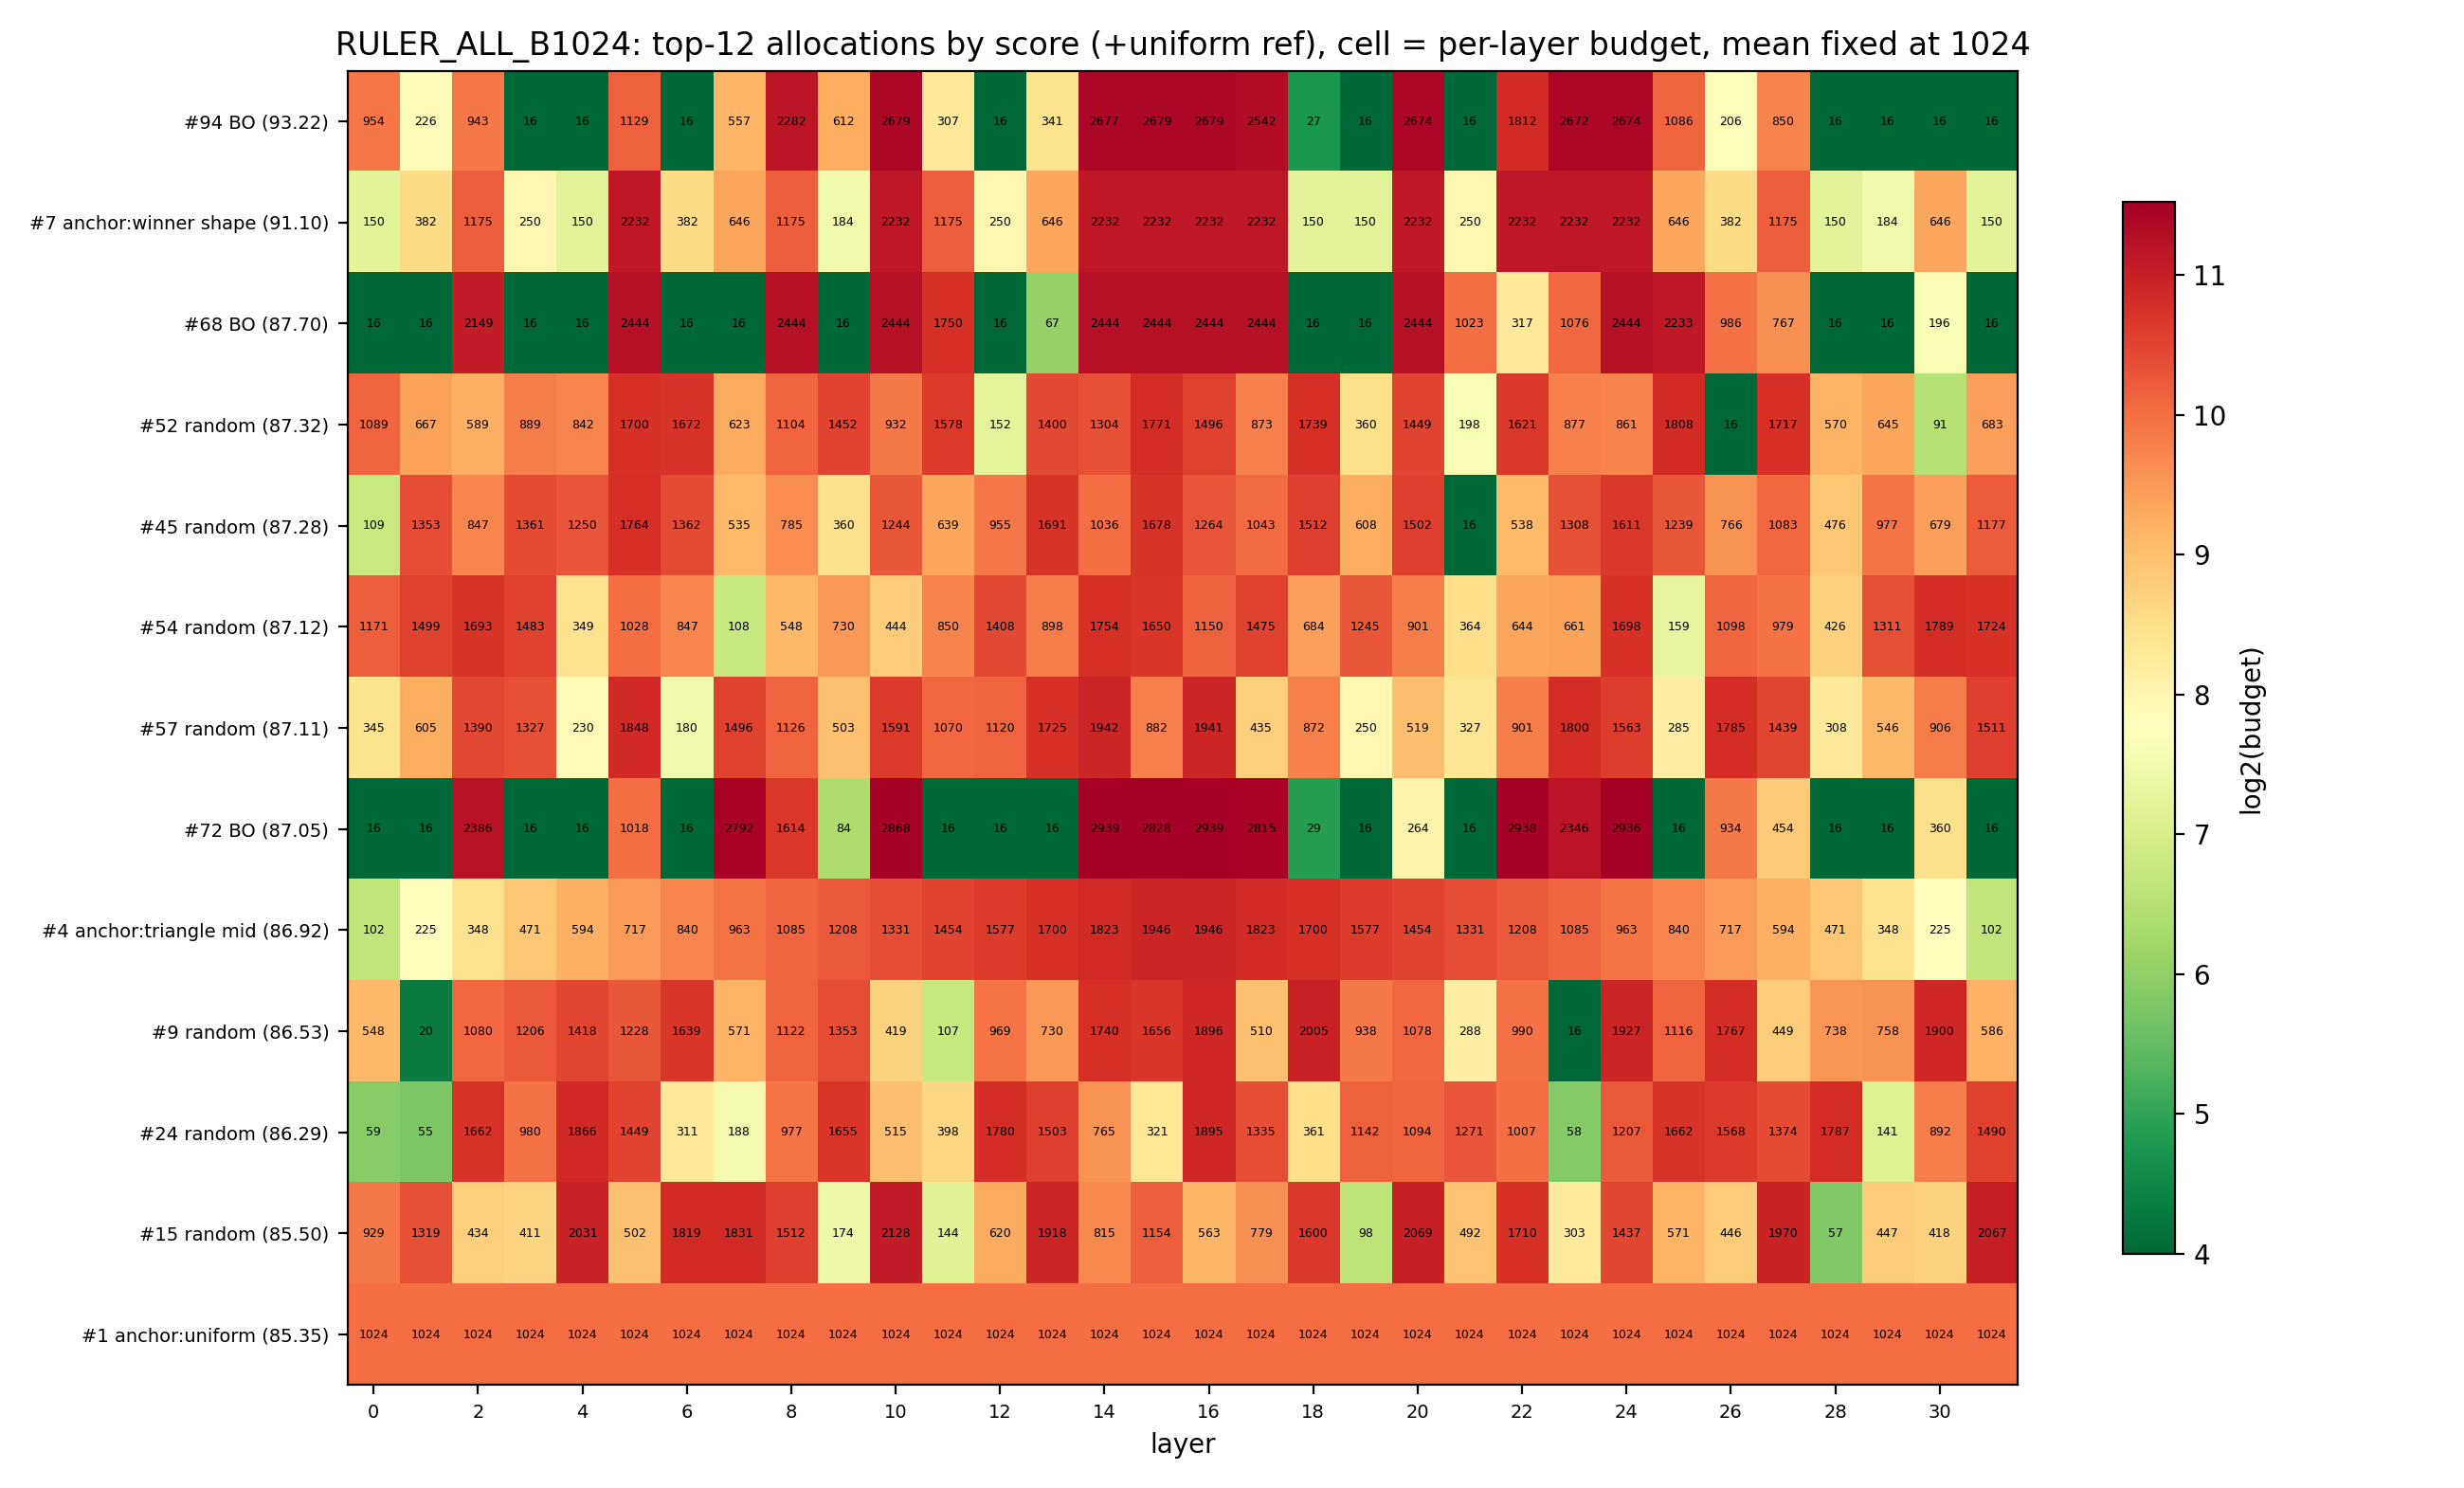
\includegraphics[width=0.95\columnwidth]{figures/figure2_heatmap.png}
  \caption{Per-layer budget allocation for five representative SnapKV configurations on RULER (B1024). Each row represents a configuration; color intensity shows the allocated budget per layer (darker = higher budget). The heatmap reveals that NAS reallocates cache strategically across layers: lower layers maintain surface-level retrieval with relatively uniform budgets, while higher layers concentrate budgets on reasoning-critical positions. The Best BO configuration (bottom row) gains +8.13 points over uniform by exploiting these layer-specific importance patterns.}
  \label{fig:heatmap}
\end{figure}

\begin{figure*}[t]
  \centering
  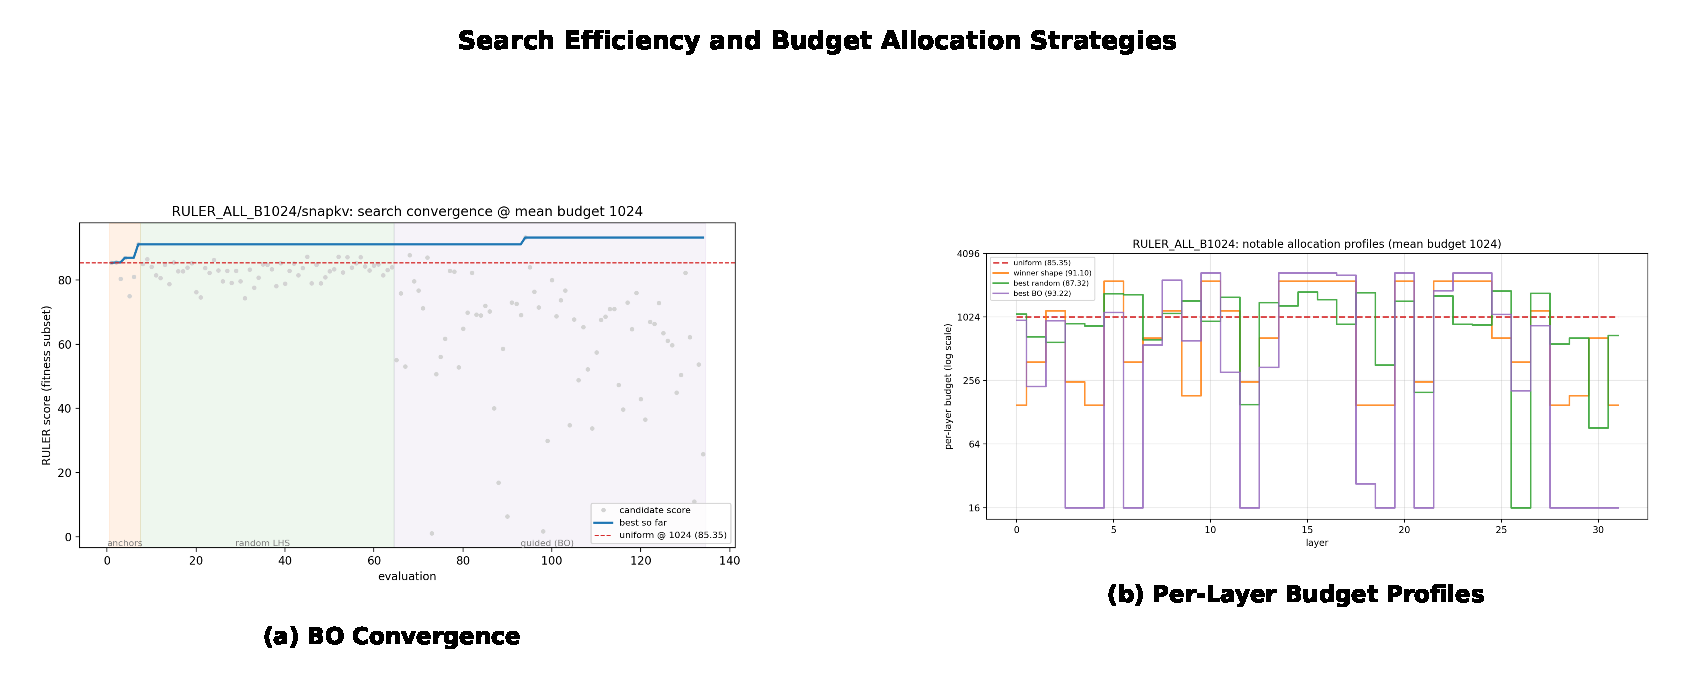
\includegraphics[width=0.95\textwidth]{figures/figure3_convergence_profiles.pdf}
  \caption{\textbf{Search Efficiency and Budget Allocation Strategies.} \textit{(a) BO Convergence:} The Bayesian optimization curve for RULER B1024 shows monotonic improvement in best score found over 200 adaptive iterations. Score jumps from initialization at iteration 0 and smoothly improves, demonstrating that surrogate-guided search efficiently explores the 32-dimensional budget space compared to random initialization alone. \textit{(b) Per-Layer Budget Profiles:} Five configurations' per-layer budget distributions across all 32 transformer layers. Uniform baseline (flat line) allocates identically to all layers; heuristic/winner/random shapes show moderate layer-wise variation from the baseline; the BO-discovered configuration (bottom, solid line with peaks) exhibits maximal strategic variation, concentrating budgets on middle-to-high layers where multi-head reasoning and token fusion dominate, and reducing budgets on lower layers handling surface-level pattern matching.}
  \label{fig:convergence}
\end{figure*}

\section{Analysis}

\begin{figure}[t]
  \centering
  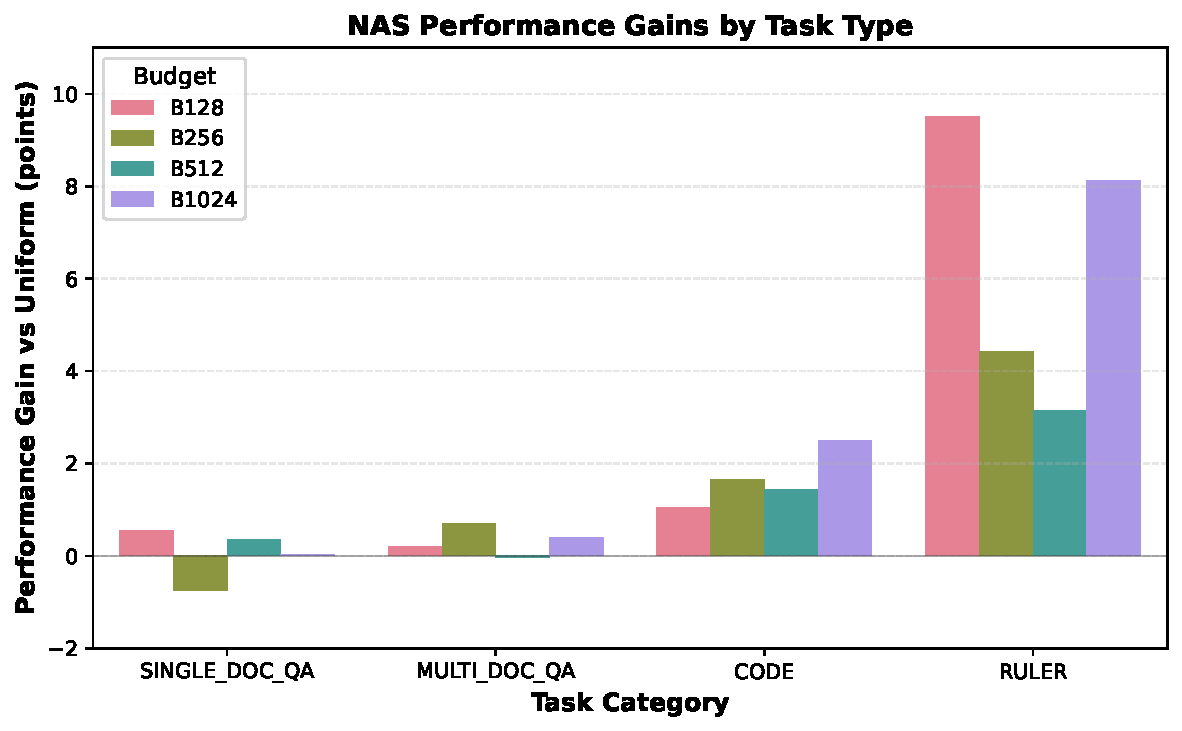
\includegraphics[width=0.95\columnwidth]{figures/figure4_task_gains.pdf}
  \caption{Performance gains of NAS best configuration over uniform allocation, by task category and budget. RULER (needle-in-haystack retrieval) shows dramatic gains (+4 to +10 points across budgets), while LongBench QA tasks show modest gains ($\leq$ 1 point). CODE tasks exhibit intermediate gains (+1 to +2.5 points). This pattern reflects task structure: RULER's positional importance is highly layer-dependent, enabling NAS to achieve substantial improvements through selective reallocation. LongBench QA distributes evidence more evenly across context, leaving less room for per-layer optimization to help.}
  \label{fig:gains}
\end{figure}

\subsection{Why Task Type Matters}

LongBench QA tasks (SINGLE\_DOC\_QA, MULTI\_DOC\_QA) treat all layers nearly equally because evidence is scattered across the context. RULER's needle-in-haystack design forces lower layers to retrieve surface tokens early and higher layers to reason; this structure gives NAS crisp layer-importance signals to optimize. Code completion exhibits intermediate behavior: function signatures and recent edits sit at predictable positions, more structured than QA but less strictly needle-like than RULER.

\subsection{Method-Specific Patterns}

H2O shows the largest absolute RULER gains (+18–33 points) because its unconstrained-search winner often overallocates to specific layers that become underfunded at low budgets; reallocation recovers this. SnapKV's gains are more modest because its simpler scoring already adapts reasonably per layer. AdaKV's per-layer adaptation means its budgets already contain layer-specific information, leaving less room for NAS to improve.

\section{Ablation: Grouped-CMA-ES}

We compare LAMP's full 32-layer search against a grouped-CMA-ES baseline inspired by EvolKV (Xu et al., EMNLP 2025), which partitions the 32 layers into 4 groups of 8 and optimizes each group independently with real CMA-ES. Evaluated on SnapKV CODE and SINGLE\_DOC\_QA at budgets 128/512/1024:

\begin{table}[t]
  \centering
  \small
  \setlength{\tabcolsep}{8pt}
  \begin{tabular}{@{} l c r r @{}}
    \toprule
    \textbf{Task} & \textbf{B} & \textbf{Grouped}$^*$ & \textbf{LAMP} \\
    \midrule
    \rowcolor{gray!10}
    CODE & 128 & 63.80 & 56.10 \\
    CODE & 512 & 65.30 & 58.17 \\
    \rowcolor{gray!10}
    CODE & 1024 & 66.34 & 58.91 \\
    SINGLE\_DOC & 128 & 43.31 & 33.67 \\
    \rowcolor{gray!10}
    SINGLE\_DOC & 512 & 43.67 & 36.33 \\
    SINGLE\_DOC & 1024 & 43.09 & 37.01 \\
    \bottomrule
  \end{tabular}
  \caption{\textbf{Ablation: Grouped-CMA-ES vs. Full Per-Layer NAS.} $^*$Grouped-CMA-ES (EvolKV-style): 4 groups of 8 layers, scored on calibration subsamples. LAMP: full 32 layers, scored on full test data. Not directly comparable; included for directional reference. Trade-off: grouped approach enables faster search but sacrifices per-layer granularity and full-data generalization.}
  \label{tab:ablation}
\end{table}

Grouped-CMA-ES achieves higher calibration-subsample scores, consistent with overfitting patterns observed elsewhere in the NAS pipeline. Full-data re-evaluation of grouped-CMA-ES is pending; results here are directional only, suggesting full per-layer search may trade calibration-time efficiency for better generalization.

\section{Limitations}

\begin{enumerate}
\item \textbf{Search cost:} LAMP requires 100–200 BO iterations per budget, incurring ~2–4 GPU-days per method/budget pair. This is amortized if applied to many workloads, but not suitable for one-off inference.
\item \textbf{Benchmark specificity:} Gains are largest on RULER (structured retrieval) and smaller on LongBench (information-spread tasks). Applicability to other long-context domains (code synthesis, summarization) requires additional benchmarking.
\item \textbf{Model scale:} Tested on Llama-3-8B only. Layer-importance patterns may differ on larger models (70B+) or other architectures (Gemma, Mistral).
\item \textbf{Eviction method dependency:} Per-layer budgets are method-specific; transferring a SnapKV-optimized config to H2O yields suboptimal results.
\end{enumerate}

\section{Conclusion}

This work demonstrates that per-layer KV-cache budget allocation, optimized via neural architecture search, can reduce memory consumption by 50–75\% while maintaining accuracy on structured retrieval tasks, with more modest but consistent gains on open-ended QA and summarization. The method is general across eviction strategies and requires no task-specific hand-tuning. Future work should explore larger models, extend to other architectures, and investigate whether learned budget patterns transfer across tasks.

\bibliography{custom}

\end{document}
